% flashcards-title: Complete groups and leftovers
% flashcards-desc: Seventeen counters are arranged as three outlined groups of five and two separately hatched leftovers.
\documentclass[dvisvgm,tikz,border=8pt]{standalone}
\usetikzlibrary{arrows.meta,patterns}

\definecolor{qraNavy}{HTML}{17324D}
\definecolor{qraBlue}{HTML}{2B6CB0}
\definecolor{qraGold}{HTML}{B7791F}
\definecolor{qraPale}{HTML}{EAF2F8}
\definecolor{qraGray}{HTML}{5C6773}

\tikzset{
  qra axis/.style={draw=qraNavy, line width=1.2pt},
  qra tick/.style={draw=qraNavy, line width=1pt},
  qra guide/.style={draw=qraGray, densely dashed, line width=0.8pt},
  qra counter/.style={circle, draw=qraNavy, fill=qraPale, line width=0.9pt, minimum size=7mm, inner sep=0pt},
  qra label/.style={font=\sffamily\bfseries, text=qraNavy},
  qra small label/.style={font=\sffamily, text=qraNavy},
}

\begin{document}
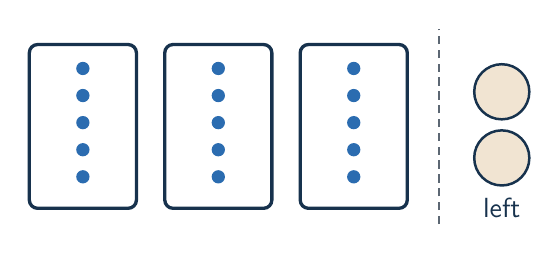
\begin{tikzpicture}[x=.8cm,y=.8cm]
  \foreach \b in {0,1,2}{\draw[qra axis,rounded corners=3pt] (\b*2.15,-.55) rectangle +(1.7,2.6);\foreach \y in {0,...,4}{\fill[qraBlue] (\b*2.15+.85,-.05+.43*\y) circle (2.4pt);}}
  \draw[qra guide] (6.5,-.8)--(6.5,2.3);
  \foreach \y in {0,1}{\node[qra counter,fill=qraGold!20] at (7.5,.25+1.05*\y) {};}
  \node[qra small label] at (7.5,-.55) {left};
\end{tikzpicture}
\end{document}
